\documentclass[12pt, a4paper]{article}
\usepackage[scaled=0.8]{FiraMono}
\usepackage{graphicx}
% The emptypage package prevents page numbers and
% headings from appearing on empty pages.
\usepackage{emptypage}
\usepackage[hscale=0.8,vscale=0.8]{geometry}
\usepackage{amsmath} % For math formatting
\usepackage{siunitx}
\usepackage{subfigure}
\usepackage{multirow}
\usepackage{booktabs}
\usepackage{listings}
\usepackage{caption}
\captionsetup[table]{position=bottom}   %% or below

\graphicspath{{images/}}


\begin{document}

\title{%
	Machine Learning and Pattern Recognition \\
	\large Project Report}

\author{Treves Mathieu - S281616}
\date{July 2024}

\maketitle
%\thispagestyle{empty}
%\clearpage

%\pagenumbering{roman} %Use lowercase Roman numerals for page numbers
%\begin{abstract}
%This is a simple paragraph at the beginning of the document. A brief introduction about the main subject.
%\end{abstract}
%\clearpage

\vspace{20 mm}

\tableofcontents
\clearpage

%\pagenumbering{arabic} % Now Use Arabic numerals for page numbers
\section{Loading and Visualizing the Dataset}
\subsection{Feature 1 - 2}

\begin{figure}[ht]
	\centering
	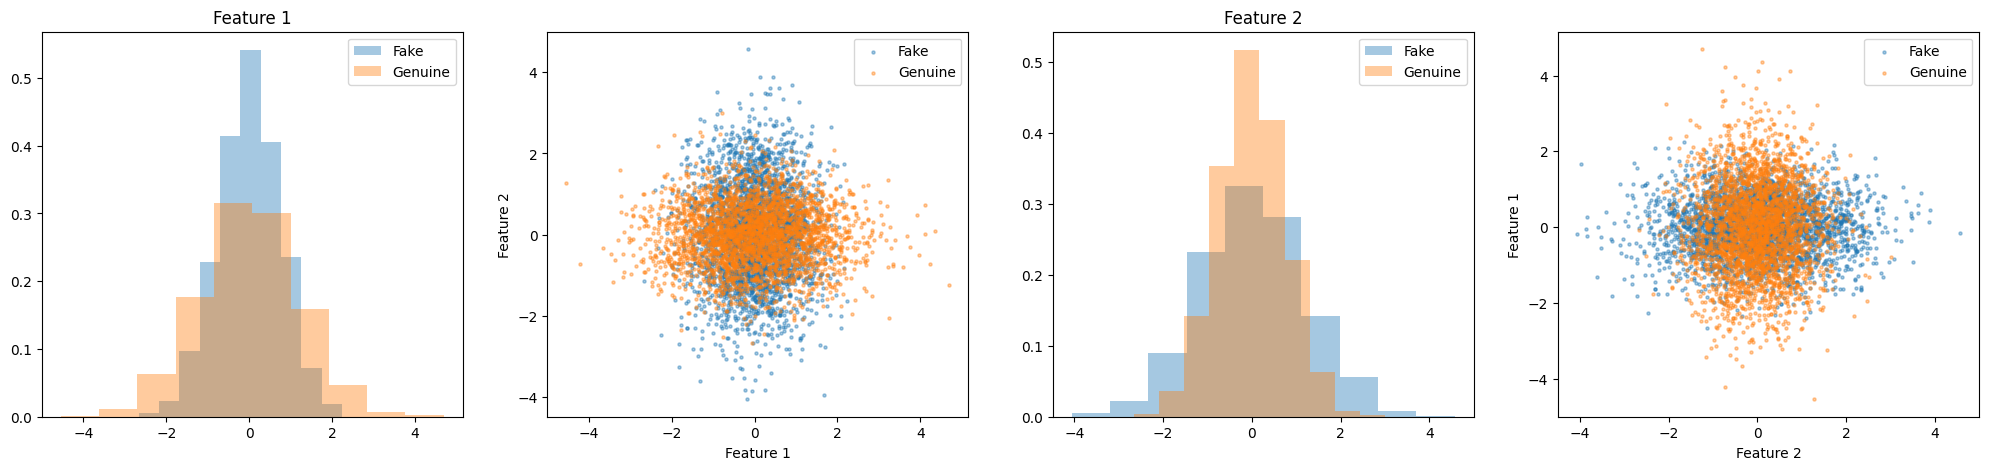
\includegraphics[width=0.8\textwidth]{features_1_2}
	\caption{Features 1 and 2}
	\label{fig:features1_2}
\end{figure}

Observing the plots for the first two features, there is a clear overlap between the two classes, in both features, especially around zero. The scatter plots show a dense region of overlap, with no clear boundary between the classes.\\
The means of the classes for feature 1 are similar, while the variances are more different, with the variance for the "Genuine" class higher that the one for the class "Fake".\\
For feature 2, the results are similar. The means are only slightly similar, with the variances that are more different, having this time the "Fake" class having a higher variance, so more spread in the data.

\begin{table}[ht!]
	\centering
	\begin{tabular}{| | c c c c c | |} 
		\hline
		Class & Mean F1 & Mean F2 & Variance F1 & Variance F2\\
		\hline\hline
 		Genuine & +0.0005 & -0.0085 & +1.4302 & +0.5783\\
 		\hline
 		Fake    & +0.0029 & +0.0187 & +0.5696 & +1.4209\\
 		\hline
 	\end{tabular}
	\caption{Mean and variance F1 + F2}
\end{table}

From the histograms, each class show an unimodal distribution for both features, with only one peak around zero.

\subsection{Feature 3 - 4}

\begin{figure}[ht]
	\centering
	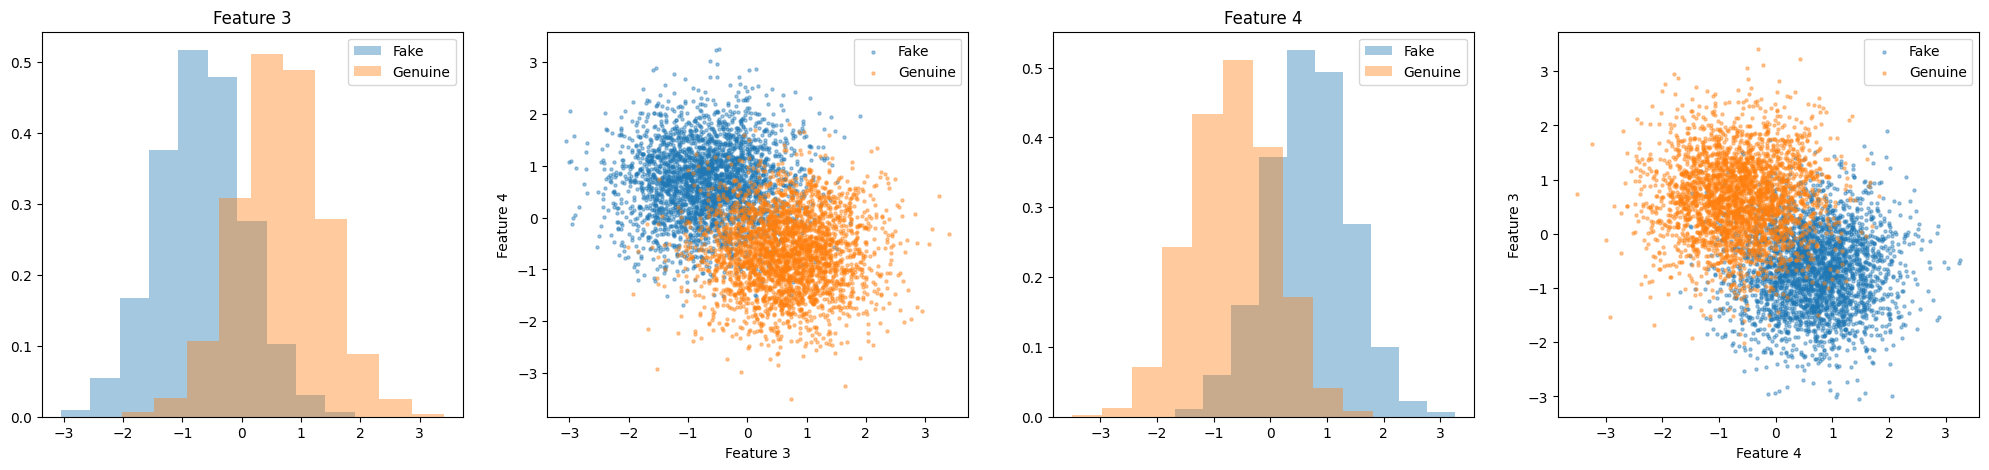
\includegraphics[width=0.8\textwidth]{features_3_4}
	\caption{Features 3 and 4}
	\label{fig:features3_4}
\end{figure}

Plotting the data for feature 3 and 4, we can see a bigger separation in respect to the previous features. There is a clear separation both in the histogram and in the scatter plots.\\
It is possible to observe a clear difference in the means, for both classes and features, similar in absolute value but with opposed sign. The variance in this case is instead similar for both classes over the two features.

\begin{table}[ht!]
	\centering
 	\begin{tabular}{| | c c c c c | |} 
 		\hline
 		Class & Mean F3 & Mean F4 & Variance F3 & Variance F4\\
 		\hline\hline
		Genuine & +0.6652 & -0.6642 & +0.5489 & +0.5533\\
 		\hline
 		Fake    & -0.6809 & +0.6708 & +0.5500 & +0.5360\\
 		\hline
 	\end{tabular}
	\caption{Mean and variance F3 + F4}
\end{table}

From the histograms, each class show an unimodal distribution for both features, but the peaks are separated for both features.

\subsection{Feature 5 - 6}

\begin{figure}[ht]
	\centering
	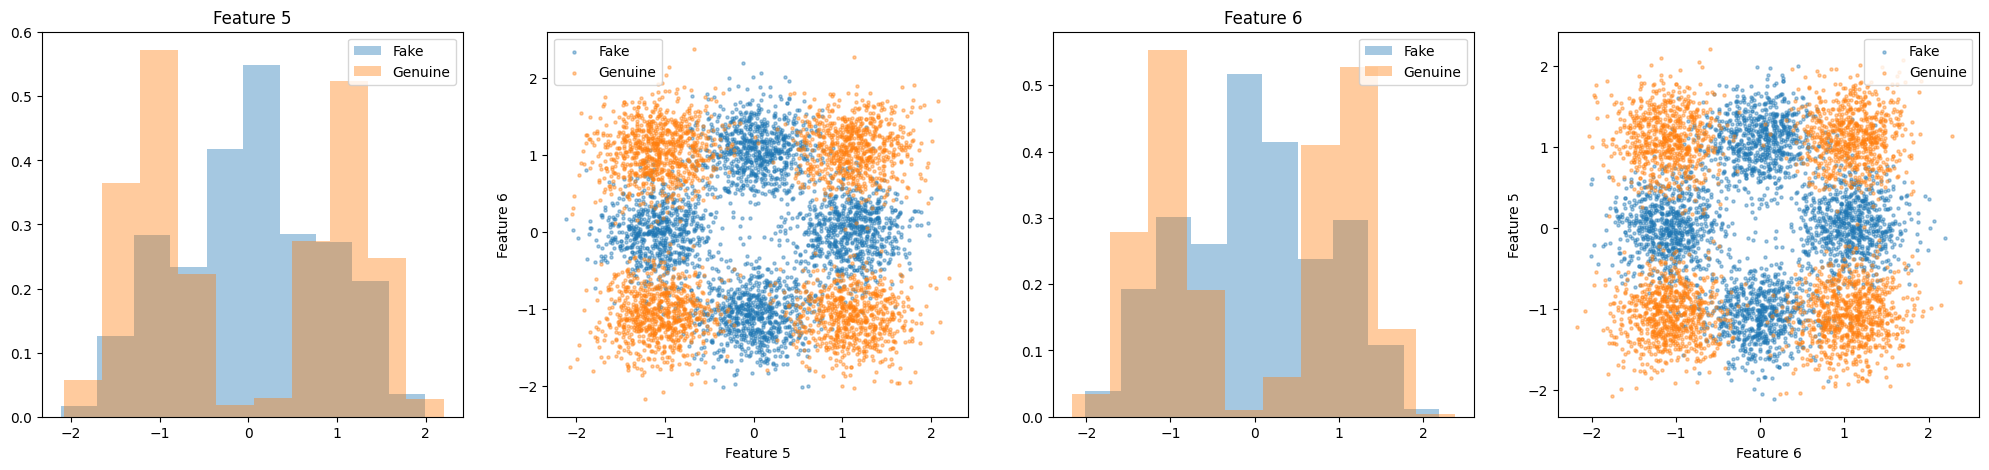
\includegraphics[width=0.8\textwidth]{features_5_6}
	\caption{Features 5 and 6}
	\label{fig:features5_6}
\end{figure}

In this case, we see a clear separation between the classes over both features. From the scatter plots it is possible to notice four different cluster for each class.\\
The means are similar, but we can see a high variance for the "Genuine" class. This is due to the fact that the "Fake" class has values in the neighbourhood of zero and one peak, and the "Genuine" class is more distant from the zero but has two nearly symmetrical peaks in the distribution.

\begin{table}[ht!]
	\centering
 	\begin{tabular}{| | c c c c c | |} 
 		\hline
 		Class & Mean F5 & Mean F6 & Variance F5 & Variance F6\\
 		\hline\hline
 		Genuine & -0.0417 & +0.0239 & +1.3178 & +1.2870\\
 		\hline
 		Fake    & +0.0280 & -0.0058 & +0.6801 & +0.7050\\
 		\hline
 	\end{tabular}
	\caption{Mean and variance F5 + F6}
\end{table}

From the histograms, the "Genuine" class shows a bimodal distribution for feature 5, and an unimodal one for feature 6. For the "Fake" class, instead, the distribution are reversed, with a bimodal one for feature 6 and an unimodal one for feature 5.

\clearpage
\section{Principal Component Analysis and Linear Discriminant Analysis}
\subsection{PCA}

In Figure \ref{fig:PCA_6_dir} it is possible to observe the results after applying PCA over all six dimensions. We can see that over the first direction, there is a smaller overlap between classes, so we can separate them better. Over all the other directions, the classes are a lot more overlapped.

\begin{figure}[ht]
	\centering
	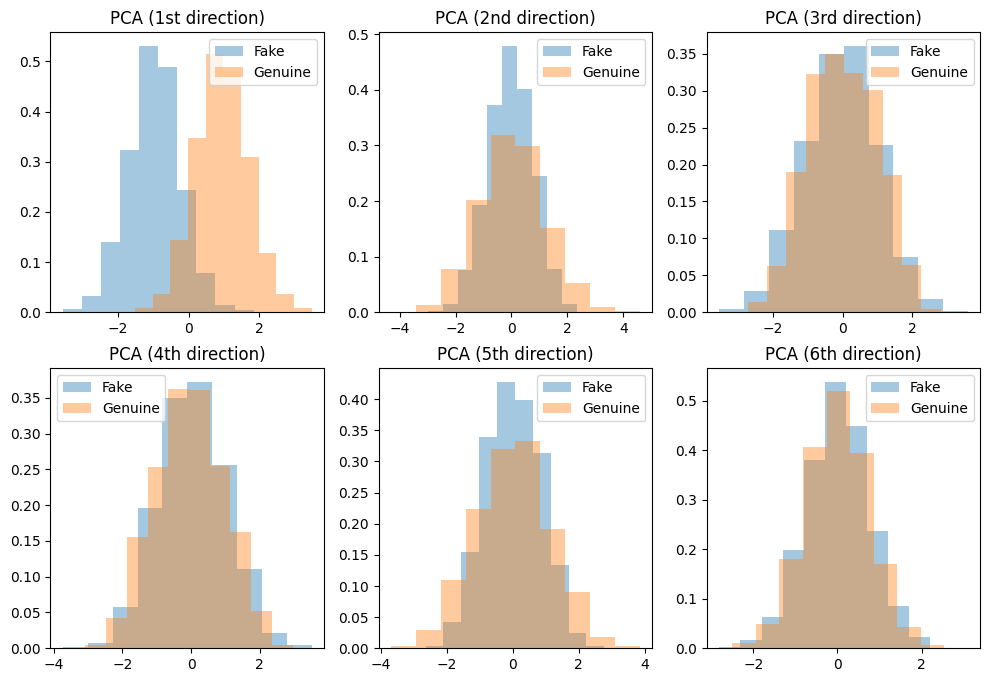
\includegraphics[width=0.8\textwidth]{PCA_6_directions}
	\caption{PCA all directions}
	\label{fig:PCA_6_dir}
\end{figure}

\subsection{LDA}

We then compute LDA over the dataset and plot the histogram, represented in Figure \ref{fig:LDA_1_dir}

\begin{figure}[ht]
	\centering
	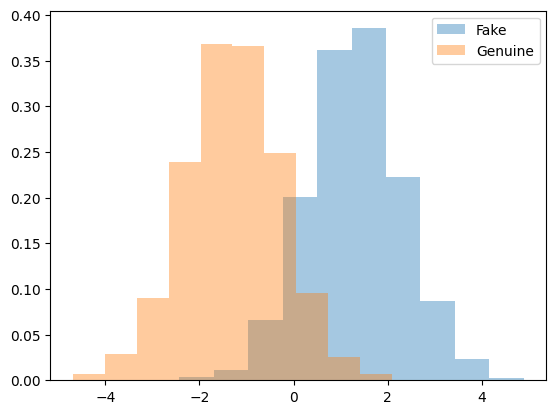
\includegraphics[width=0.4\textwidth]{LDA_1_direction}
	\caption{LDA}
	\label{fig:LDA_1_dir}
\end{figure}

We can see that LDA finds a good direction and is able to separate a lot the two classes. The overlap, from a first view, is similar to the one of the first PCA direction, and a lot better from all the others.

\subsection{LDA as classifier}

Dividing the dataset in model training and validation sets, and applying LDA,we can compute the predictions and the error rate. With the default threshold, calculated as

\begin{lstlisting}[xleftmargin=.1\textwidth]
(DTR[0, LTR==0].mean() + DTR[0, LTR==1].mean()) / 2.0
\end{lstlisting}

\noindent we find a 9.30\% error rate. If we tweak a little the threshold - by iterating over multiple values in the class overlap interval - we can find a better value that gives an er of 9.05\%.

\begin{table}[ht!]
	\centering
 	\begin{tabular}{| | c c | |} 
 		\hline
		Threshold & Error rate\\
		\hline\hline
		-0.018 & 9.30\%\\
		\hline
		-0.106 & \textbf{9.05\%}\\
		\hline
	\end{tabular}
	\caption{Error rates}
\end{table}

\subsection{PCA + LDA}

We can then try to apply PCA and LDA at the same time. We do PCA over the model training data, and then we apply LDA to classify the validation data. in Figure \ref{fig:PCA+LDA} we can observe the histogram representing the separation of the classes after applying both PCA and LDA.

\begin{figure}[ht]
	\centering
	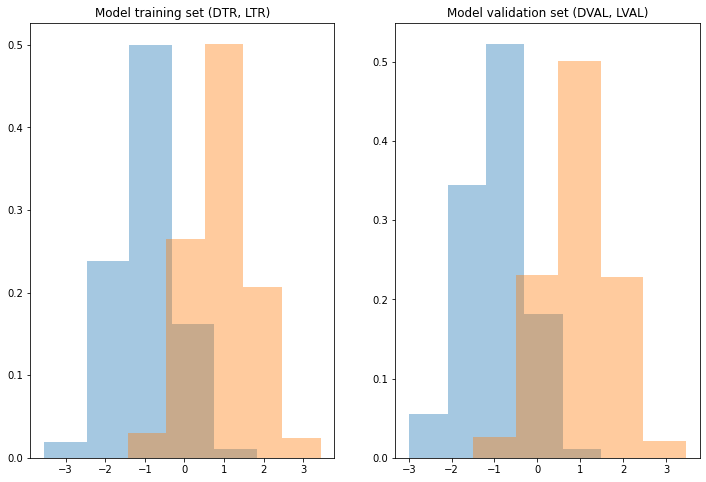
\includegraphics[width=0.8\textwidth]{PCA+LDA}
	\caption{PCA+LDA}
	\label{fig:PCA+LDA}
\end{figure}

If we try some combinations of PCA over a variable number of dimensions, we find that the best performance we can get is with \textbf{m=2}. We can see that choosing to do the PCA over 1 dimension, we actually get a better error rate, at 8.85\%, but then LDA is irrelevant.

\begin{table}[ht!]
	\centering
 	\begin{tabular}{| | c c c | |} 
 		\hline
 		PCA dim & error rate & best thresh\\
 		\hline\hline
 		1 & 8.85\% & +0.013\\
 		\hline
 		2 & \textbf{8.95\%} & -0.033\\
 		\hline
 		3 & 9.15\% & -0.057\\
 		\hline
 		4 & 9.10\% & -0.062\\
 		\hline
 		5 & 9.05\% & -0.095\\
 		\hline
 		6 & 9.05\% & -0.106\\
 		\hline
 	\end{tabular}
	\caption{Error rates different PCA dimensions}
\end{table}

\hfill \break
\noindent So, we find that applying PCA before doing LDA is beneficial for this task.

\clearpage
\section{Computing Probability densities}
\subsection{Plot Gaussian densities}

For each class, for each component of the feature vector of that class, we compute the ML estimate for the parameters of a 1D Gaussian distribution. In Figure \ref{fig:MVG_6_features} we can see the plot the distribution density on top of the normalized histograms of the two classes, for each feature.

\begin{figure}[ht]
	\centering
	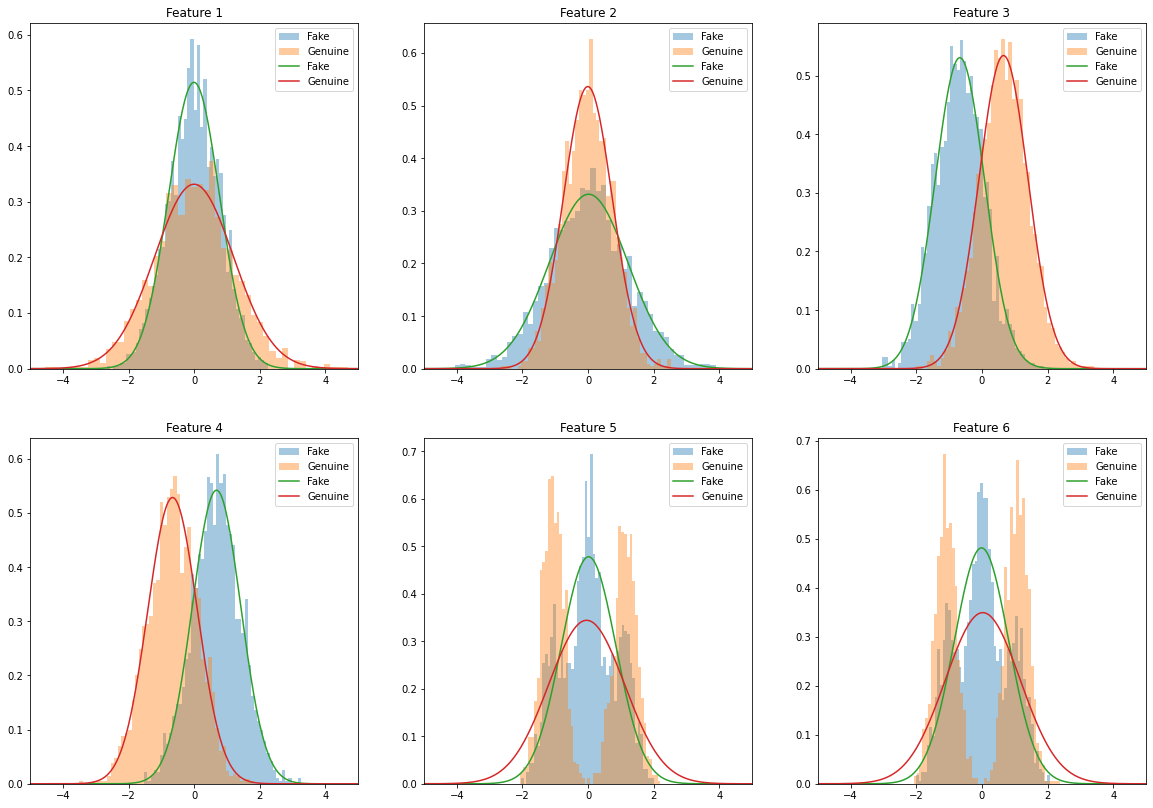
\includegraphics[width=.9\textwidth]{MVG_6_features}
	\caption{MVG for all features}
	\label{fig:MVG_6_features}
\end{figure}

We can observe that the Gaussian densities provide a good fit for feature 1 to 4. Instead, for feature 5 and 6, the Gaussian model is significantly less accurate, at least for the \textit{Genuine} class, probably because it has two peaks.

\clearpage
\section{Generative models for classification}
\subsection{Trying different models}

We can try three different classifiers: Multivariate Gaussian Classifier (MVG), Tied MVG and Naive Bayes Gaussian Classifier. If we apply all of them to the data, we obtain the following error rates. We can see that the best model is MVG, instead the Naive Bayes one is the one performing worse.
	
\begin{table}[ht!]
	\centering
 	\begin{tabular}{| | c c | |} 
 		\hline
 		Model & Error rate\\
 		\hline\hline
 		MVG & 7.0\%\\
 		\hline
 		Tied MVG & 7.2\%\\
 		\hline
 		Naive Bayes & 9.3\%\\
 		\hline
 	\end{tabular}
	\caption{Error rate different models}
\end{table}

Now we extract the covariance matrices for class 0 and 1 from the MVG model parameters. These matrices contain, on the diagonal, the variances of the different features, and the elements outside the diagonal are the feature co-variances. We can observe that for either classes, the features co-variances are usually smaller than the variances.

\begin{table}[ht!]
	\centering
    \begin{tabular}{| | c c c c c c | |} 
 		\hline
    	6.009e-01 & 5.158e-05 & 1.905e-02 & 1.925e-02 & 1.280e-02 & -1.347e-02\\
 		\hline
    	5.158e-05 & 1.447e+00 & -1.613e-02 & -1.585e-02 & -2.645e-02 & 2.291e-02\\
 		\hline
    	1.905e-02 & -1.613e-02 & 5.653e-01 & -1.843e-03 & -6.914e-03 & 1.689e-02\\
 		\hline
    	1.925e-02 & -1.585e-02 & -1.843e-03 & 5.416e-01 & 5.251e-03 & 1.357e-02\\
 		\hline
    	1.280e-02 & -2.6451e-02 & -6.914e-03 & 5.251e-03 & 6.960e-01 & 1.584e-02\\
 		\hline
    	-1.347e-02 & 2.291e-02 & 1.689e-02 & 1.357e-02 & 1.584e-02 & 6.865e-01\\
 		\hline
 	\end{tabular}
    \caption{Covariance matrix class 0}
\end{table}

\begin{table}[ht!]
	\centering
    \begin{tabular}{| | c c c c c c | |} 
 		\hline
    	1.448e+00 & -1.472e-02 & 5.570e-03 & 1.574e-02 & 1.950e-02 & -1.767e-04\\
 		\hline
    	-1.472e-02 & 5.534e-01 & -1.122e-02 & -9.065e-03 & -1.466e-02 & 1.635e-02\\
 		\hline
    	5.570e-03 & -1.122e-02 & 5.575e-01 & 2.756e-02 & -3.770e-03 & -1.460e-02\\
 		\hline
    	1.574e-02 & -9.065e-03 & 2.756e-02 & 5.697e-01 & -1.170e-02 & 3.499e-02\\
 		\hline
    	1.950e-02 & -1.466e-02 & -3.770e-03 & -1.170e-02 & 1.342e+00 & 1.695e-02\\
 		\hline
    	-1.767e-04 & 1.635e-02 & -1.460e-02 & 3.499e-02 & 1.695e-02 & 1.304e+00\\
 		\hline
 	\end{tabular}
    \caption{Covariance matrix class 1}
\end{table}

To better visualize the strength of covariances with respect to variances we can compute, the Pearson correlation coefficient. The correlation matrix has diagonal elements equal to 1, whereas out-of diagonal elements correspond to the correlation coefficients for all feature pairs, with values from -1 to 1. When the element in the matrix is equal to 0, the features are uncorrelated, whereas values close to +-1 denote strong correlation.

\begin{table}[ht!]
	\centering
    \begin{tabular}{| | c c c c c c | |} 
 		\hline
 		\textbf{1.00} & 0.00 & 0.03 & 0.03 & 0.02 & -0.02 \\ 
 		\hline
 		0.00 & \textbf{1.00} & -0.02 & -0.02 & -0.03 & 0.02 \\
 		\hline
 		0.03 & -0.02 & \textbf{1.00} & -0.00 & -0.01 & 0.03 \\
 		\hline
 		0.03 & -0.02 & -0.00 & \textbf{1.00} & 0.01 & 0.02 \\
 		\hline
 		0.02 & -0.03 & -0.01 & 0.01 & \textbf{1.00} & 0.02 \\
 		\hline
 		-0.02 & 0.02 & 0.03 & 0.02 & 0.02 & \textbf{1.00} \\
 		\hline
 	\end{tabular}
\end{table}

\begin{table}[ht!]
	\centering
    \begin{tabular}{| | c c c c c c | |} 
 		\hline
 		\textbf{1.00} & -0.02 & 0.01 & 0.02 & 0.01 & -0.00 \\ 
 		\hline
 		-0.02 & \textbf{1.00} & -0.02 & -0.02 & -0.02 & 0.02 \\
 		\hline
 		0.01 & -0.02 & \textbf{1.00} & 0.05 & -0.00 & -0.02 \\
 		\hline
 		0.02 & -0.02 & 0.05 & \textbf{1.00} & -0.01 & 0.04 \\
 		\hline
 		0.01 & -0.02 & -0.00 & -0.01 & \textbf{1.00} & 0.01 \\
 		\hline
 		-0.00 & 0.02 & -0.02 & 0.04 & 0.01 & \textbf{1.00} \\
 		\hline
 	\end{tabular}
    \caption{Pearson Correlation Coefficient Matrix for Class 0 and 1}
\end{table}

From these matrices, we can see that most off-diagonal entries are close to 0, for the two classes, which suggests that most features are very weakly correlated with each other. The Naive Bayes classifier operates under the assumption that the features are conditionally independent given the class, so the weak correlations observed in both classes are beneficial.


\subsection{Analysis using features 1-6}

From the analysis done in the previous parts, it appears that the Gaussian assumption holds reasonably well for Features 2 and 3, is acceptable for Features 1 and 4, and does not fit well for Features 5 and 6. These features that show significant deviations from the Gaussian curves, like multiple peaks or asymmetry, indicate that the Gaussian model might be overly simplistic for these dimensions and might not provide accurate predictions or classifications based on these features alone.

\begin{table}[ht!]
	\centering
 	\begin{tabular}{| | c c c c | |} 
 		\hline
 		Features & MVG & Naive Bayes & Tied MVG\\
 		\hline\hline
 		1-6 & 7.00\% & 7.00\% & 9.30\%\\
 		\hline
 	\end{tabular}
	\caption{Error rates with features 1,2,3,4,5,6}
\end{table}

\subsection{Analysis using features 1-4}

To analyse if indeed the last set of features negatively affects our classifier because of poor modelling assumptions, we can try repeating the classification using only feature 1 to 4. We can see that, despite discarding the worse features, the model does not improve its accuracy (neither three of the models used).

\begin{table}[ht!]
	\centering
 	\begin{tabular}{| | c c c c | |} 
 		\hline
 		Features & MVG & Naive Bayes & Tied MVG\\
 		\hline\hline
 		1-4 & 7.95\% & 7.65\% & 9.50\%\\
 		\hline
 	\end{tabular}
	\caption{Error rates with features 1,2,3,4}
\end{table}

\subsection{Analysis using features 1-2}

We found that for features 1 and 2 means are similar but variances are not, so we try to model using only these two features. In this case, the MVG and Naive Bayes models perform similarly. The Tied MVG model instead has a much higher error rate. This suggests that for these features - where the means are similar but variances differ - using a tied covariance matrix results in a loss of important discriminatory information that is preserved in the distinct covariance matrices of the standard MVG model.

\begin{table}[ht!]
	\centering
 	\begin{tabular}{| | c c c c | |} 
 		\hline
 		Features & MVG & Naive Bayes & Tied MVG\\
 		\hline\hline
 		1-2 & 36.50\% & 36.30\% & 49.45\%\\
 		\hline
 	\end{tabular}
	\caption{Error rates with features 1-2}
\end{table}

\subsection{Analysis using features 3-4}

We found that for features 3 and 4 means are different and variances are similar, so we try to model using only these two features. In this case, all models show very similar performance, with a marginal advantage to the Tied MVG model. This slight improvement in the Tied MVG model could be attributed to the fact that for these features the variances are similar. Thus, using a tied covariance matrix doesn't affect the model's performance and might even simplify the model.

\begin{table}[ht!]
	\centering
 	\begin{tabular}{| | c c c c | |} 
 		\hline
 		Features & MVG & Naive Bayes & Tied MVG\\
 		\hline\hline
 		3-4 & 9.45\% & 9.45\% & 9.40\%\\
 		\hline
 	\end{tabular}
	\caption{Error rates with features 3-4}
\end{table}

\subsection{Using PCA as preprocessing}

Finally, we can analyze the effects of PCA as pre-processing, using it to reduce the dimensionality of the feature space before applying the three models. We find that PCA is not too much effective in reducing the error rates over this dataset. In some cases, it improves a little over applying only the model without preprocessing, but in general the best - mean - performances can be seen without PCA.

\begin{table}[ht!]
	\centering
 	\begin{tabular}{| | c c c c | |} 
 		\hline
 		PCA dim & MVG & Naive Bayes & Tied MVG\\
 		\hline\hline
 		1 & 9.25\% & 9.25\% & 9.35\%\\
 		\hline
 		2 & 8.80\% & 8.85\% & \textbf{9.25\%}\\
 		\hline
 		3 & 8.80\% & 9.00\% & \textbf{9.25\%}\\
 		\hline
 		4 & 8.05\% & 8.85\% & \textbf{9.25\%}\\
 		\hline
 		5 & 7.10\% & 8.75\% & 9.30\%\\
 		\hline
 		6 & \textbf{7.00\%} & 8.90\% & 9.30\%\\
 		\hline
 		\hline
 		NO PCA & \textbf{7.00\%} & \textbf{7.00\%} & 9.30\%\\
 		\hline 
 	\end{tabular}
	\caption{Error rates with PCA pre-processing}
\end{table}

\section{Performance of Multivariate Gaussian models}
\subsection{Computing minDCF and actDCF}

We now analyze the performance of the MVG classifier and its variants for different applications, focusing on three main ones, with effective priors equal to 0.1, 0.5 and 0.9. Since we are using effective priors, the cost of errors will be considered equal to 1.

In the following tables, there are presented the computation of minimum and actual DCF across the three different models: MVG, Tied MVG and Naive Bayes. Each model has been analyzed using PCA as preprocessing with different number of dimensions. The deviation of the actual DCF from the minimum DCF has also been computed.

\begin{table}[ht!]
	\centering
	\begin{tabular}{| | c c c c c c | |}
		\hline
		Model & Prior & PCA Dim & Min DCF & Act DCF & aDCF/mDCF \\
		\hline\hline
		MVG & 0.1 & 1 & 0.3686 & 0.3970 & \textbf{07.69\%} \\
		\hline
		MVG & 0.1 & 2 & 0.3526 & 0.3879 & 10.00\% \\
		\hline
		MVG & 0.1 & 3 & 0.3563 & 0.3879 & 08.86\% \\
		\hline
		MVG & 0.1 & 4 & 0.3012 & 0.3529 & 17.17\% \\
		\hline
		MVG & 0.1 & 5 & 0.2738 & \textbf{0.3041} & 11.07\% \\
		\hline
		MVG & 0.1 & 6 & \textbf{0.2629} & 0.3051 & 16.06\% \\
		\hline\hline
		MVG & 0.5 & 1 & 0.1769 & 0.1850 & 04.58\% \\
		\hline
		MVG & 0.5 & 2 & 0.1731 & 0.1760 & 01.68\% \\
		\hline
		MVG & 0.5 & 3 & 0.1734 & 0.1759 & \textbf{01.42\%} \\
		\hline
		MVG & 0.5 & 4 & 0.1537 & 0.1609 & 04.69\% \\
		\hline
		MVG & 0.5 & 5 & 0.1331 & 0.1419 & 06.59\% \\
		\hline
		MVG & 0.5 & 6 & \textbf{0.1302} & \textbf{0.1399} & 07.50\% \\
		\hline\hline
		MVG & 0.9 & 1 & 0.4342 & 0.4775 & 09.98\% \\
		\hline
		MVG & 0.9 & 2 & 0.4384 & 0.4434 & \textbf{01.15\%} \\
		\hline
		MVG & 0.9 & 3 & 0.4392 & 0.4680 & 06.56\% \\
		\hline
		MVG & 0.9 & 4 & 0.4150 & 0.4598 & 10.79\% \\
		\hline
		MVG & 0.9 & 5 & 0.3512 & \textbf{0.3980} & 13.33\% \\
		\hline
		MVG & 0.9 & 6 & \textbf{0.3423} & 0.4001 & 16.87\% \\
		\hline
	\end{tabular}
	\caption{MVG model performance}
\end{table}

We find that the MVG model with PCA = 6 is the best performing one over the three in exam, for our main application (with $\tilde{\pi} = 0.1$). We can also see that when reducing the dimensionality of the dataset using PCA gives us values of the actual DCF that are more similar to the ones of the minimum one. Increasing the dimensionality instead lead to bigger deviations.
The model is not too much consistent across the different applications, having best results when using a $\tilde{\pi} = 0.5$, followed by $\tilde{\pi} = 0.1$ and lastly by $\tilde{\pi} = 0.9$.

In the following two tables, containing the results for the Tied MVG and Naive Bayes models, we have a similar situation. We see that the models perform more equally across all the PCA applications, but as the MVG one, for every prior we have different performances. The models are well calibrated for the $\tilde{\pi} = 0.5$ configuration, and a bit less for the other twos. 

\clearpage

\begin{table}[ht!]
	\centering
	\begin{tabular}{| | c c c c c c | |}
		\hline
		Model & Prior & PCA Dim & Min DCF & Act DCF & aDCF/mDCF \\
		\hline\hline
		Tied MVG & 0.1 & 1 & 0.3686 & 0.4021 & \textbf{09.07\%} \\
		\hline
		Tied MVG & 0.1 & 2 & 0.3630 & \textbf{0.3960} & 09.09\% \\
		\hline
		Tied MVG & 0.1 & 3 & 0.3681 & 0.4082 & 10.89\% \\
		\hline
		Tied MVG & 0.1 & 4 & \textbf{0.3610} & 0.4031 & 11.66\% \\
		\hline
		Tied MVG & 0.1 & 5 & 0.3648 & 0.4051 & 11.03\% \\
		\hline
		Tied MVG & 0.1 & 6 & 0.3628 & 0.4061 & 11.91\% \\
		\hline\hline
		Tied MVG & 0.5 & 1 & \textbf{0.1769} & 0.1870 & 05.72\% \\
		\hline
		Tied MVG & 0.5 & 2 & 0.1789 & \textbf{0.1850} & 03.45\% \\
		\hline
		Tied MVG & 0.5 & 3 & 0.1830 & \textbf{0.1850} & \textbf{01.08\%} \\
		\hline
		Tied MVG & 0.5 & 4 & 0.1821 & \textbf{0.1850} & 01.60\% \\
		\hline
		Tied MVG & 0.5 & 5 & 0.1812 & 0.1860 & 02.69\% \\
		\hline
		Tied MVG & 0.5 & 6 & 0.1812 & 0.1860 & 02.64\% \\
		\hline\hline
		Tied MVG & 0.9 & 1 & \textbf{0.4342} & 0.4806 & 10.68\% \\
		\hline
		Tied MVG & 0.9 & 2 & 0.4352 & 0.4785 & 09.96\% \\
		\hline
		Tied MVG & 0.9 & 3 & \textbf{0.4342} & \textbf{0.4565} & 05.14\% \\
		\hline
		Tied MVG & 0.9 & 4 & 0.4441 & 0.4615 & 03.92\% \\
		\hline
		Tied MVG & 0.9 & 5 & 0.4451 & 0.4626 & \textbf{03.91\%} \\
		\hline
		Tied MVG & 0.9 & 6 & 0.4421 & 0.4626 & 04.63\% \\
		\hline
	\end{tabular}
	\caption{Tied MVG model performance}
\end{table}

\begin{table}[ht!]
	\centering
	\begin{tabular}{| | c c c c c c | |}
		\hline
		Model & Prior & PCA Dim & Min DCF & Act DCF & aDCF/mDCF \\
		\hline\hline
		Naive Bayes & 0.1 & 1 & 0.3686 & 0.3970 & \textbf{07.69\%} \\
		\hline
		Naive Bayes & 0.1 & 2 & 0.3562 & \textbf{0.3869} & 08.63\% \\
		\hline
		Naive Bayes & 0.1 & 3 & 0.3645 & 0.3950 & 08.36\% \\
		\hline
		Naive Bayes & 0.1 & 4 & 0.3614 & 0.3970 & 09.84\% \\
		\hline
		Naive Bayes & 0.1 & 5 & 0.3545 & 0.3930 & 10.87\% \\
		\hline
		Naive Bayes & 0.1 & 6 & \textbf{0.3535} & 0.3920 & 10.90\% \\
		\hline\hline
		Naive Bayes & 0.5 & 1 & 0.1769 & 0.1850 & 04.58\% \\
		\hline
		Naive Bayes & 0.5 & 2 & \textbf{0.1710} & 0.1770 & 03.48\% \\
		\hline
		Naive Bayes & 0.5 & 3 & 0.1746 & 0.1799 & 03.04\% \\
		\hline
		Naive Bayes & 0.5 & 4 & 0.1717 & 0.1770 & 03.09\% \\
		\hline
		Naive Bayes & 0.5 & 5 & 0.1737 & \textbf{0.1750} & \textbf{00.75\%} \\
		\hline
		Naive Bayes & 0.5 & 6 & 0.1727 & 0.1780 & 03.07\% \\
		\hline\hline
		Naive Bayes & 0.9 & 1 & 0.4342 & 0.4775 & 09.98\% \\
		\hline
		Naive Bayes & 0.9 & 2 & 0.4323 & \textbf{0.4424} & \textbf{02.33\%} \\
		\hline
		Naive Bayes & 0.9 & 3 & 0.4343 & 0.4591 & 05.70\% \\
		\hline
		Naive Bayes & 0.9 & 4 & \textbf{0.4313} & 0.4630 & 07.35\% \\
		\hline
		Naive Bayes & 0.9 & 5 & 0.4340 & 0.4660 & 07.37\% \\
		\hline
		Naive Bayes & 0.9 & 6 & 0.4359 & 0.4512 & 03.50\% \\
		\hline
	\end{tabular}
	\caption{Naive Bayes model performance}
\end{table}

\clearpage

\subsection{Bayes error plots}
We now compute the Bayes error plot and visualize the minimum and actual DCF for a range of applications, in particular considering prior log odds in the range (-4,+4). We do this for all three models.

\begin{figure}[ht]
    \centering
    \subfigure[]{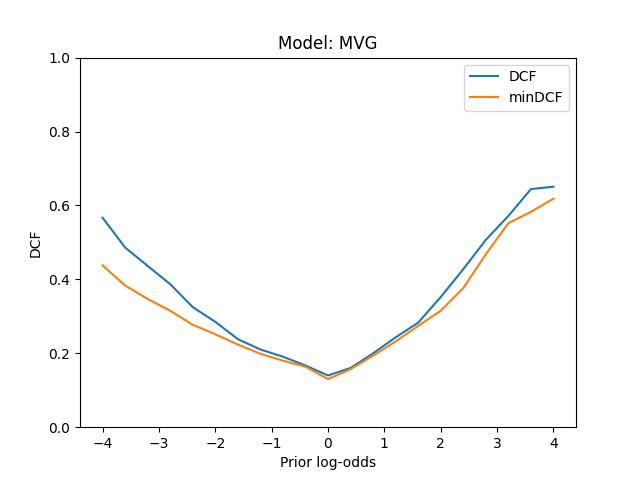
\includegraphics[width=0.45\textwidth]{project07/DCF_MVG}} 
    \subfigure[]{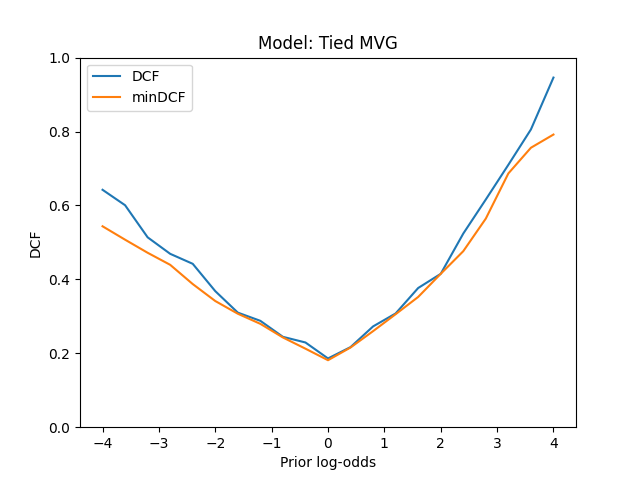
\includegraphics[width=0.45\textwidth]{project07/DCF_TMVG}} 
    \subfigure[]{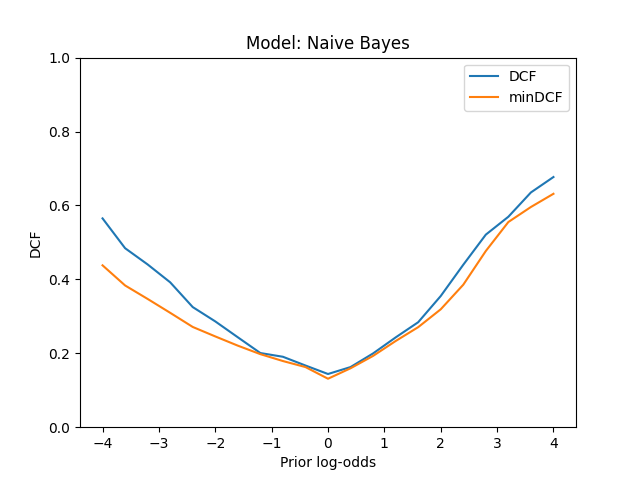
\includegraphics[width=0.45\textwidth]{project07/DCF_NB}}
    \caption{(a) MVG (b) Tied MVG (c) NB}
    \label{fig:DCF_models}
\end{figure}

We can see that the three models are well calibrated, at least in the (-1,+1) range, with similar values for minimum and actual DCF. When considering the low and high limits of the range, all three models have poor performances, with the values of minimum DCF worsening and the ones for the actual DCF beginning to deviate a lot from the optimal ones.

\clearpage

\section{Performance of Logistic Regression models}
We now analyze the binary logistic regression model on our data. We want to try different values for $\lambda$, in this case from $\num{e-4}$ to $\num{e2}$. The plots of actual and minimum DCF over lambda are proposed in the following pages, and also different techniques are tried to process the data before the regularization.

\subsection{Standard version}

\begin{figure}[ht]
	\centering
	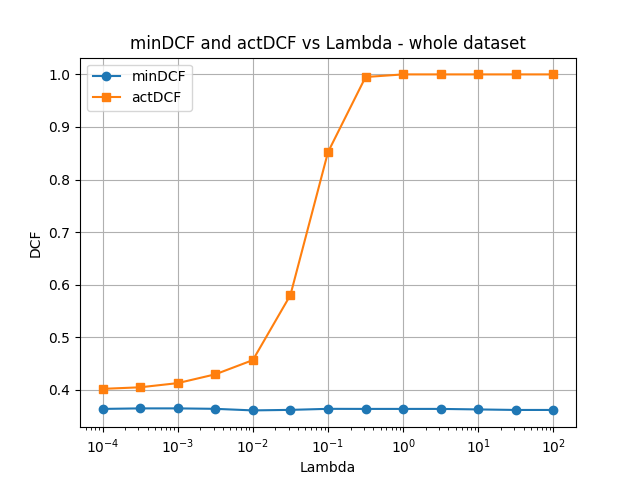
\includegraphics[width=.4\textwidth]{project08/dcf_lambda_whole}
	\caption{DCF over lambda - whole dataset}
	\label{fig:LR_whole}
\end{figure}

From this plot we can see that as $\lambda$ increases from $\num{e-3}$ to $\num{e0}$, actDCF starts to increase sharply. This can suggests that the model becomes over-regularized, leading to poor generalization and higher DCF on the validation set. When increasing even more the value of the regularization coefficient, actDCF plateaus around 1.0, indicating very poor performance, likely due to excessive regularization. The value of minDCF remains instead relatively constant. The optimal range for $\lambda$ is around $\num{e-4}$ to $\num{e-3}$, where actDCF is minimized.

\subsection{Fewer training samples version}
We now plot the relationship between the regularization coefficient and the two metrics when training the model on a smaller dataset (keeping only 1 out of 50 training samples).

\begin{figure}[ht]
	\centering
	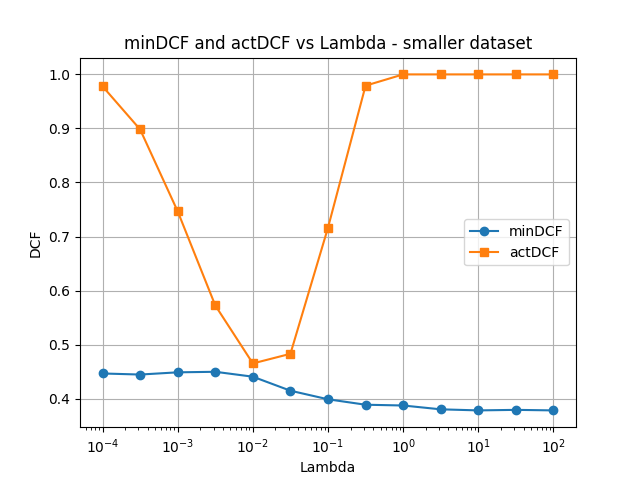
\includegraphics[width=.4\textwidth]{project08/dcf_lambda_smaller}
	\caption{DCF over lambda - smaller dataset}
	\label{fig:LR_smaller}
\end{figure}

We can now see that the model perform a lot worse for smaller values of $\lambda$, having optimal performances only in a small window around $\lambda = \num{e-2}$.
The explanation for this is likely that with a smaller training dataset, the model is more prone to overfitting due to the limited amount of data to learn from. Regularization helps mitigate overfitting by imposing a penalty on the complexity of the model, thus obtaining some balance. Moreover, when $\lambda$ is too high, the model is overly constrained, leading to underfitting where the model cannot capture the patterns in the data, resulting in higher actDCF.

\subsection{Prior-weighted model}

\begin{figure}[ht]
	\centering
	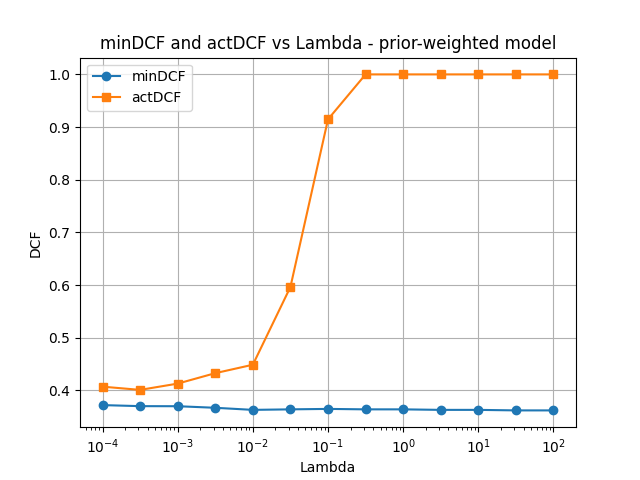
\includegraphics[width=.4\textwidth]{project08/dcf_lambda_wheighted}
	\caption{DCF over lambda - prior-weighted dataset}
	\label{fig:LR_priorWeighted}
\end{figure}

The shape of the curves is similar to the non-prior-weighted model trained on the full dataset, with actDCF increasing sharply for higher values of $\lambda$, while minDCF remains constant. The prior-weighted model, however, requires knowledge of the target prior during training, which may not always be available or accurate, so in this case it may be best to use the standard model. 

\subsection{Quadratic Logistic Regression model}

\begin{figure}[ht]
	\centering
	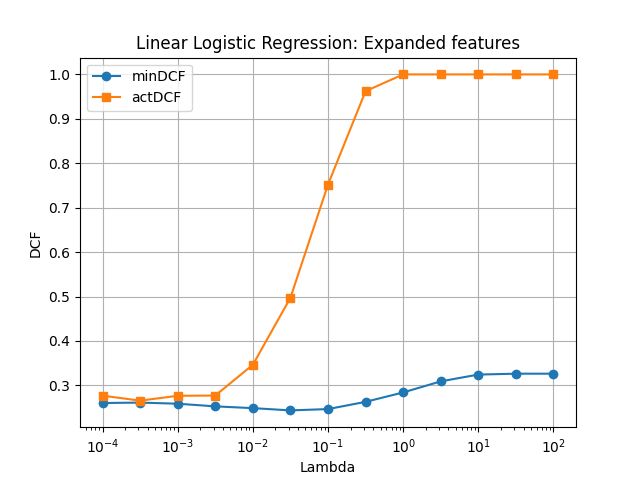
\includegraphics[width=.4\textwidth]{project08/dcf_lambda_expandedFeatures}
	\caption{DCF over lambda - expanded features}
	\label{fig:LR_expandedFeatures}
\end{figure}

In this case, we see that the regularization is more effective than for the other models, at least for smaller values of $\lambda$. Both the actual and minimum DCF, for $\lambda < \num{e-2}$, have values in the vicinity of 0.3, instead of 0.4. Moreover, we see that the gap between minDCF and actDCF is a lot smaller, indicating that our model can perform nearly optimally. As $\lambda$ increases, we obtain values similar to the ones obtained from the linear models.

\subsection{Centering the model}
When centering or applying Z-normalization, we see that the model performs not too differently that without these techniques, as the original features were already almost standardized.

\begin{figure}[ht]
    \centering
    \subfigure[]{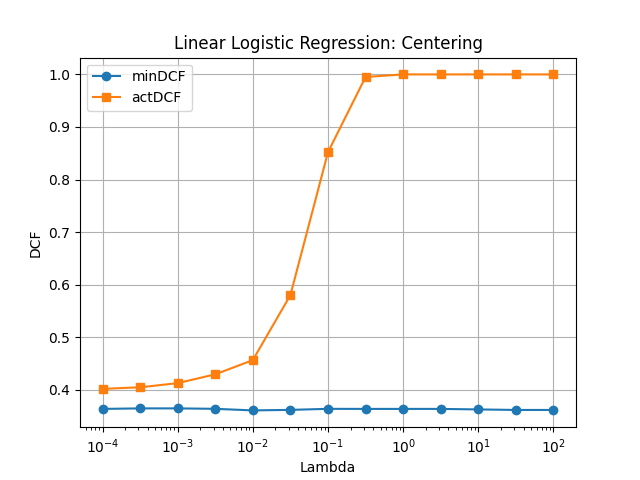
\includegraphics[width=0.4\textwidth]{project08/dcf_lambda_centering}} 
    \subfigure[]{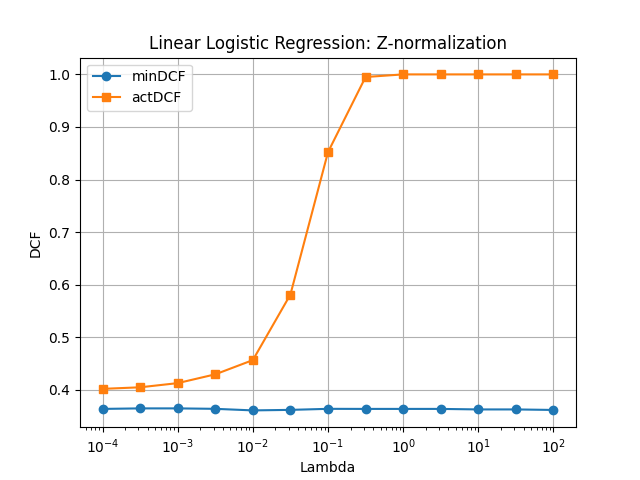
\includegraphics[width=0.4\textwidth]{project08/dcf_lambda_zNorm}}
    \caption{(a) Centering (b) Z-Normalization}
    \label{fig:LR_affine}
\end{figure}

\subsection{LR vs Gaussian Models}
After these analysis, we can compare what minDCF and actDCF we obtain with the best values of $\lambda$ for the different models.

\begin{table}[ht!]
	\centering
 	\begin{tabular}{| | c c c c | |} 
 		\hline
 		Model & $\lambda$ & Min DCF & Act DCF\\
 		\hline\hline
 		Whole & $\num{10e-2}$ & 0.3611 & 0.4568\\
 		\hline
 		Smaller & $\num{10e1}$ & 0.3783 & 1.0000\\
 		\hline
 		Prior-weight & $\num{3.162e2}$ & 0.3620 & 1.0000\\
 		\hline
 		QLR & $\num{3.162e-2}$  & \textbf{0.2436} & 0.4972\\
 		\hline
 		Center & $\num{10e-2}$ & 0.3611 & 0.4568\\
 		\hline
 		Z-norm & $\num{10e-2}$ & 0.3611 & 0.4568\\
 		\hline
 	\end{tabular}
	\caption{Best values models}
\end{table}

We can see that the \textbf{Quadratic Logistic Regression} with expanded features performs significantly better than the other models, that all have similar performance, at least considering the minimum DCF. Its actDCF is significantly higher, indicating potential mis-calibration.

If we compare this results with the ones from the previous part, with the Gaussian Models, we can appreciate how the QLR model, at least for our target application ($\tilde{\pi} = 0.1$), performs better with the optimal value for the regularization coefficient. The effectiveness of the QLR model suggests that the dataset could contains non-linear relationships that can be better captured by quadratic terms in the logistic regression model.


\section{Performance of Support Vector Machines models}
Now, we try applying SVM to the data, using different models and iterating over different hyper-parameters to find the most suitable ones for the target application ($\tilde{\pi} = 0.1$).


\subsection{Linear model}
First, we train a linear SVM model, trying with and without centering the data. We iterate over different values of C to find the best one. For C, we use log-spaced values given by numpy.logspace(-5, 0, 11).

\begin{figure}[ht]
    \centering
    \subfigure[]{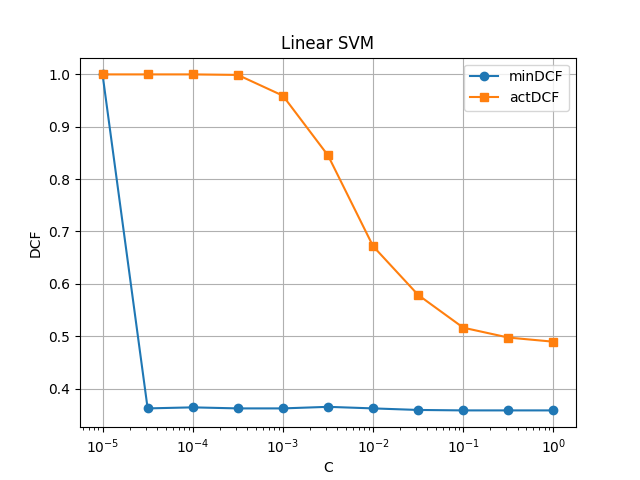
\includegraphics[width=0.4\textwidth]{project09/svm_linear}} 
    \subfigure[]{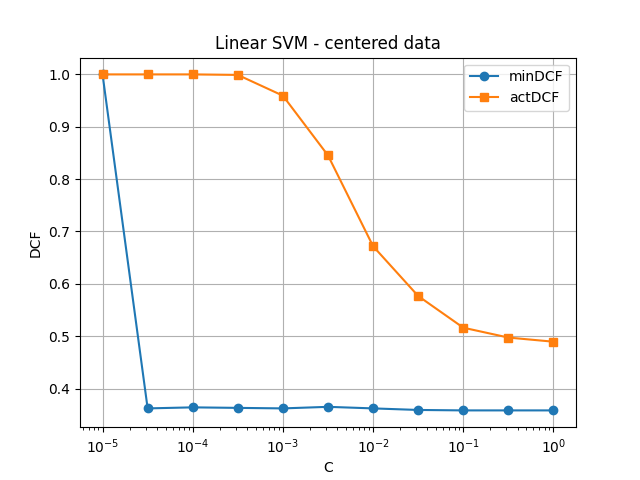
\includegraphics[width=0.4\textwidth]{project09/svm_linear_centered}}
    \caption{(a) SVM Linear (b) SVM Linear centered data}
    \label{fig:SVM_Linear}
\end{figure}

We can see that the regularization coefficient C has a minimal effect on minDCF scores, with scores that remain relatively stable. For the actDCF, C has a significant effect on the scores. As C increases (regularization weakens), actDCF scores decrease sharply, especially in the range of $\num{e-3}$ to $\num{e-1}$. The model achieves its best performance (lowest actDCF) with weak regularization (high C values).
The large gap between minDCF and actDCF, especially for small C values, suggests that the scores are not well-calibrated for the target application.
While analyzing the model with centered data, the situation is the same and the plot does not changes.

\subsection{Polynomial Kernel}
We now consider the polynomial kernel. For simplicity, we consider only the kernel with d = 2; c = 1, and we set $\xi$ = 0, since the kernel already implicitly accounts for the bias term (due to c = 1).

\begin{figure}[ht]
	\centering
	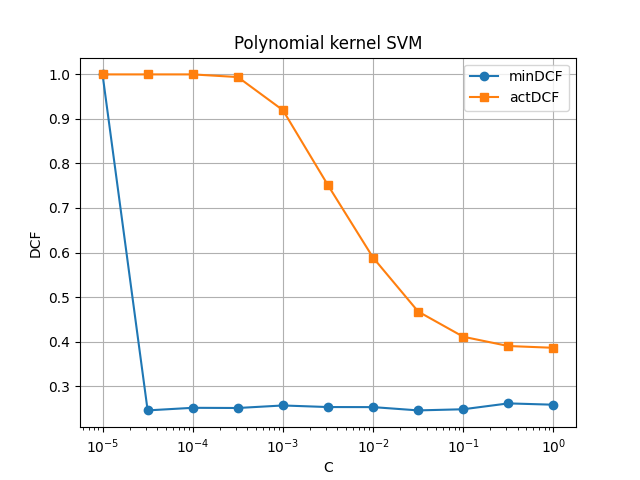
\includegraphics[width=.4\textwidth]{project09/svm_poly_kernel}
	\caption{SVM with Polynomial Kernel}
	\label{fig:SVM_Poly}
\end{figure}

Similarly to the linear model, the regularization coefficient C has a minimal effect on minDCF scores, with scores that remain relatively stable. For the actDCF, C has a more significant effect.
In comparison to the linear SVM, though, the minDCF and actDCF scores (with high C values) are lower, indicating better overall discriminative power. The improved performance suggests that the quadratic model can capture more complex decision boundaries than the linear SVM, which is beneficial for this particular dataset. We saw the same results when training linear regression models, when the quadratic one (using a dataset with expanded features) was the overall best.

\subsection{Radial Basis Function Kernel}
For RBF kernel we need to optimize both $\gamma$ and C (since the RBF kernel does not implicitly account for the bias term we set $\xi$ = 1). We adopt a grid search approach, i.e., we consider different values of  $\gamma$ and different values of C, and try all possible combinations. For  $\gamma$ we analyze values $\gamma \in \{e^{-4}, e^{-3}, e^{-2}, e^{-1}\}$ , while for C we use log-spaced values given by numpy.logspace(-3, 2, 11).

\begin{figure}[ht]
	\centering
	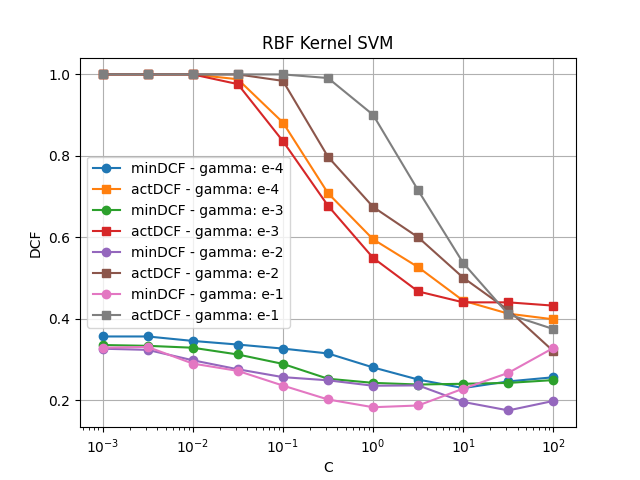
\includegraphics[width=.4\textwidth]{project09/svm_rbf_kernel}
	\caption{SVM with RBF kernel}
	\label{fig:SVM_RBF}
\end{figure}

As for the other models, as C increases, both minDCF and actDCF generally decrease, a trend that can be seen for all gamma values. We can see that lower gamma values $e^{-4}, e^{-3}$ tend to perform better than higher values $e^{-2}, e^{-1}$, especially for the actDCF. The best performance appears to be achieved with $\gamma = e^{-3}$ (but not for our target application, as can be seen in the results table, that benefits from a value of $\gamma = e^{-3}$), and high C values, from $\num{e1}$ to $\num{e2}$.

In regard to the calibration of the model, it seems better than linear SVM but similar to polynomial kernel SVM. But there is still a gap between minDCF and actDCF, indicating imperfect calibration.

The RBF kernel's success suggests the dataset may have: a) Non-linear decision boundaries b) Potentially clustered or localized patterns in the feature space c) Complex interactions between features that benefit from the infinite-dimensional mapping of RBF.

\subsection{Results}
In the following table, there are provided the results for all the SVM models tried, computing the values of minimum DCF and actual DCF for out target application. The best model is the RBF kernel one, with the polynomial kernel as second best.

\begin{table}[ht!]
	\centering
 	\begin{tabular}{| | c c c c c c c c | |} 
 		\hline
 		Model & C & d & c & $\xi$ & $\gamma$ & Min DCF & Act DCF \\
 		\hline\hline
 		Linear & 0.1 & - & - & - & - & 0.3582 & 0.5162\\
 		\hline
 		Linear centered & 0.1 & - & - & - & - & 0.3582 & 0.5162\\
 		\hline
 		Poly & $\num{3.162e-2}$ & 2 & 1 & 0 & - & 0.2455 & 0.4674\\
 		\hline
 		RBF & $\num{3.162e2}$ & - & - & 1 & $e^{-4}$ & \textbf{0.1755} & \textbf{0.4216}\\
 		\hline
 	\end{tabular}
	\caption{Best values models}
\end{table}

\clearpage

\section{Performance of Gaussian Mixture Models}

\subsection{Performance of GMM}

\begin{table}[ht!]

    \centering
    \begin{minipage}{.5\textwidth}
		\centering
 		\begin{tabular}{|| c c c c ||} 
 			\hline
 			\multicolumn{4}{|| c ||}{ GMM Type: FullCov }\\
 			numC0 & numC1 & Min DCF & Act DCF \\
 			\hline\hline
1 & 1     & 0.2629 & 0.3051\\
\hline
1 & 2     & 0.2649 & 0.3051\\
\hline
1 & 4     & 0.2139 & 0.2368\\
\hline
1 & 8     & 0.1850 & 0.1957\\
\hline
1 & 16    & \textbf{0.1495} & 0.2055\\
\hline
1 & 32    & 0.1847 & 0.2273\\
\hline
2 & 1     & 0.2181 & 0.2317\\
\hline
2 & 2     & 0.2160 & 0.2337\\
\hline
2 & 4     & 0.2234 & 0.2255\\
\hline
2 & 8     & 0.1860 & 0.2133\\
\hline
2 & 16    & 0.1701 & 0.1980\\
\hline
2 & 32    & 0.1857 & 0.2269\\
\hline
4 & 1     & 0.2330 & 0.2458\\
\hline
4 & 2     & 0.2317 & 0.2357\\
\hline
4 & 4     & 0.2161 & 0.2395\\
\hline
4 & 8     & 0.1887 & 0.2064\\
\hline
4 & 16    & 0.1745 & 0.1871\\
\hline
4 & 32    & 0.1867 & 0.2380\\
\hline
8 & 1     & 0.1759 & 0.2004\\
\hline
8 & 2     & 0.1808 & 0.1913\\
\hline
8 & 4     & 0.1959 & 0.1989\\
\hline
8 & 8     & 0.1786 & 0.1928\\
\hline
8 & 16    & 0.1526 & \textbf{0.1725}\\
\hline
8 & 32    & 0.1755 & 0.1903\\
\hline
16 & 1    & 0.1670 & 0.1783\\
\hline
16 & 2    & 0.1657 & 0.1753\\
\hline
16 & 4    & 0.1918 & 0.1918\\
\hline
16 & 8    & 0.1755 & 0.2050\\
\hline
16 & 16   & 0.1631 & 0.1766\\
\hline
16 & 32   & 0.1752 & 0.1955\\
\hline
32 & 1    & 0.2570 & 0.2580\\
\hline
32 & 2    & 0.2560 & 0.2600\\
\hline
32 & 4    & 0.2460 & 0.2825\\
\hline
32 & 8    & 0.2191 & 0.2251\\
\hline
32 & 16   & 0.1938 & 0.2180\\
\hline
32 & 32   & 0.2337 & 0.2499\\
\hline
 		\end{tabular}
		\caption{GMM FullCov}
    \end{minipage}%
    \begin{minipage}{.5\textwidth}
		\centering
 		\begin{tabular}{|| c c c c ||} 
 			\hline
 			\multicolumn{4}{|| c ||}{ GMM Type: Diagonal }\\
 			numC0 & numC1 & Min DCF & Act DCF \\
 			\hline\hline
1 & 1     & 0.2570 &  0.3022\\
\hline
1 & 2     & 0.2605 &  0.3051\\
\hline
1 & 4     & 0.2098 &  0.2258\\
\hline
1 & 8     & 0.2045 &  0.2207\\
\hline
1 & 16    & 0.1433 &  0.1807\\
\hline
1 & 32    & 0.1373 &  0.1967\\
\hline
2 & 1     & 0.2449 &  0.2716\\
\hline
2 & 2     & 0.2489 &  0.2674\\
\hline
2 & 4     & 0.1990 &  0.2099\\
\hline
2 & 8     & 0.2039 &  0.2089\\
\hline
2 & 16    & 0.1536 &  0.1731\\
\hline
2 & 32    & 0.1436 &  0.1810\\
\hline
4 & 1     & 0.1451 &  0.1501\\
\hline
4 & 2     & 0.1542 &  0.1611\\
\hline
4 & 4     & 0.1481 &  0.1687\\
\hline
4 & 8     & 0.1403 &  0.1515\\
\hline
4 & 16    & 0.1372 &  0.1687\\
\hline
4 & 32    & 0.1412 &  0.1677\\
\hline
8 & 1     & 0.1731 &  0.1763\\
\hline
8 & 2     & 0.1762 &  0.1874\\
\hline
8 & 4     & 0.1585 &  0.1838\\
\hline
8 & 8     & 0.1463 &  0.1809\\
\hline
8 & 16    & 0.1324 &  \textbf{0.1487}\\
\hline
8 & 32    & \textbf{0.1312} &  0.1517\\
\hline
16 & 1    & 0.2069 &  0.2217\\
\hline
16 & 2    & 0.2039 &  0.2217\\
\hline
16 & 4    & 0.1963 &  0.2050\\
\hline
16 & 8    & 0.1979 &  0.2140\\
\hline
16 & 16   & 0.1622 &  0.1769\\
\hline
16 & 32   & 0.1644 &  0.1799\\
\hline
32 & 1    & 0.1748 &  0.1964\\
\hline
32 & 2    & 0.1748 &  0.1974\\
\hline
32 & 4    & 0.1929 &  0.1979\\
\hline
32 & 8    & 0.1929 &  0.1989\\
\hline
32 & 16   & 0.1850 &  0.2069\\
\hline
32 & 32   & 0.1766 &  0.1989\\
\hline
 		\end{tabular}
		\caption{GMM Diagonal}
    \end{minipage}
\end{table}

We train a full covariance model and a diagonal one. For each one, we have to find the optimal number of components for the two classes, so we try every possible combination in (limiting ourself to 32 components).

We find that, for both models, increasing the number of components for class 1, increases the performances, decreasing the values of the DCFs, especially for the minimum one. Instead, increasing the number of components for class 0, does not have a strong correlation to an increase of the performance of the model.

Both full covariance and diagonal model performs similarly, with the diagonal one having best results in general. The latter one is also the best model when selecting a number of components equals to 8 for C0 and 32 for C1, and it is the model we choose.

\subsection{Analysis between models}
In this section, we compare the three best models chosen in the previous parts: QLR, SVM with RBF kernel and diagonal GMM. All the values are computer respect to the target application ($\tilde{\pi} = 0.1$).

\begin{table}[ht!]
	\centering
 	\begin{tabular}{| | c c c | |} 
 		\hline
 		Model & Min DCF & Act DCF\\
 		\hline\hline
 		QLR & 0.2436 & 0.4972\\
 		\hline
 		SVM & 0.1755 & 0.4216\\
 		\hline
 		GMM & \textbf{0.1312} & \textbf{0.1517}\\
 		\hline
 	\end{tabular}
	\caption{Best values models}
\end{table}

We see that the best performing model, especially in terms of actual DCF, is the GMM one. Also, this is the best calibrated one (we'll see that is also well calibrated over a wide range of applications).

\begin{figure}[ht]
    \centering
    \subfigure[]{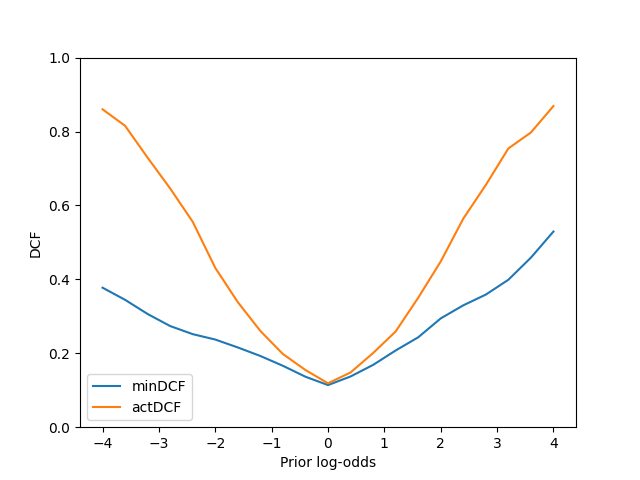
\includegraphics[width=0.5\textwidth]{project10/lr_bayes}} 
    \subfigure[]{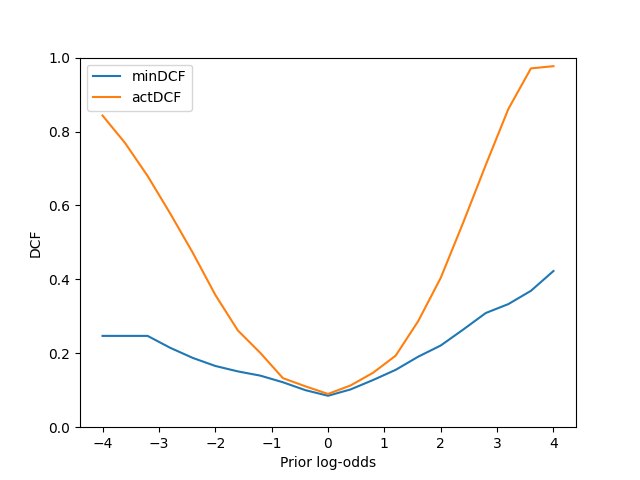
\includegraphics[width=0.5\textwidth]{project10/svm_bayes}}
    \subfigure[]{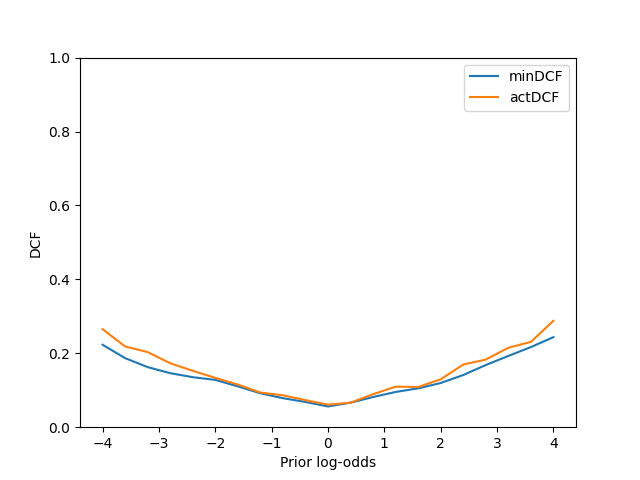
\includegraphics[width=0.5\textwidth]{project10/gmm_bayes}}
    \caption{(a) QLR (b) SVM RBF (c) GMM }
    \label{fig:Bayes plot all models}
\end{figure}

If we now plot the Bayes error (we plot over log-odds ranging from -4 to +4), we can compare the performance of these models for different applications. 

We see that, as we already seen for our target application, the GMM model is the best performing one, having low minimum DCF and actual DCF over the whole range, presenting also very little mis-calibration.

The LR and SVM models, instead, have actual DCF values that are a lot different from minimum DCF ones, so showing that they are not so well calibrated. In general, we see poorer performances, even theoretical ones if we watch the values of the minDCF.
\clearpage

\section{Calibration and Fusion}

\subsection{Models calibration}
We now compute a calibration transformation for the scores of the best-performing classifier we selected earlier. We test different priors for training the logistic regression model, and evaluate the performance of the calibration transformation in terms of actual DCF for the target application.

In the following table, we can see the performance of the three models, in terms of minimum and actual DCF for our target application ($\tilde{\pi} = 0.1$).

\begin{table}[ht!]
	\centering
 	\begin{tabular}{| | c c | c c | c c | |} 
 		\hline
 		Model & $\pi$ & Min DCF & Act DCF & cal. Min DCF & cal. Act DCF\\
 		\hline\hline
 		QLR & 0.7 & 0.2436 & 0.4972 & 0.2448 & 0.2458\\
 		\hline
 		SVM & 0.2 & 0.1755 & 0.4216 & 0.1775 & 0.1823\\
 		\hline
 		GMM & 0.1 & 0.1312 & 0.1517 & 0.1342 & 0.1478\\
 		\hline
 	\end{tabular}
	\caption{Model calibration}
\end{table}

We can see that for every model, calibrating it improves its performance, even drastically when considering the LR and SVM models. The GMM one was already well calibrated from the start, but we see an increase in its performance when considering the actDCF.

\begin{figure}[ht]
    \centering
    \subfigure[]{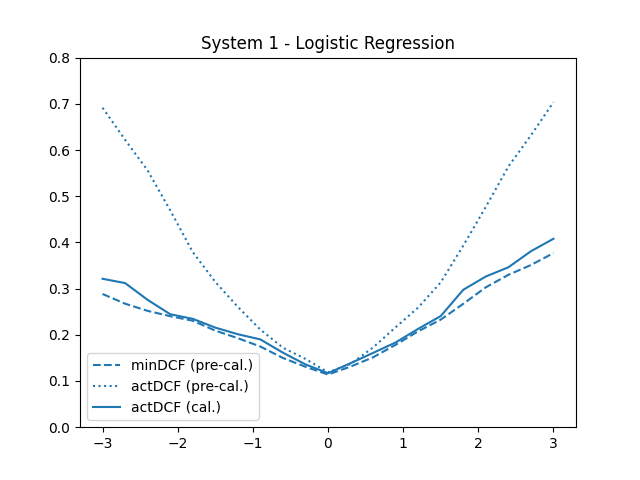
\includegraphics[width=0.4\textwidth]{project11/project11_LR}} 
    \subfigure[]{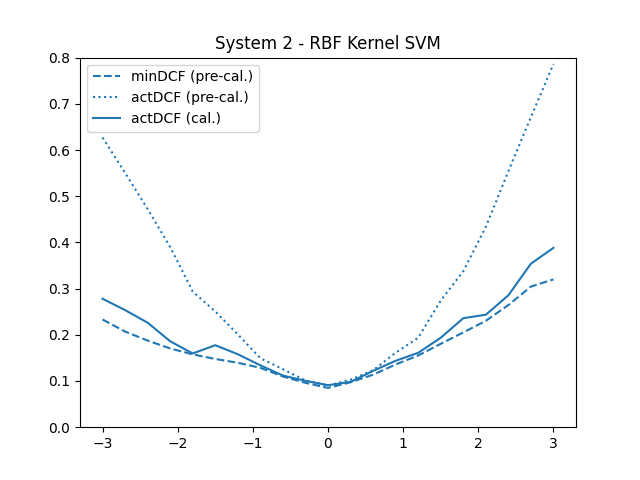
\includegraphics[width=0.4\textwidth]{project11/project11_SVM}}
    \subfigure[]{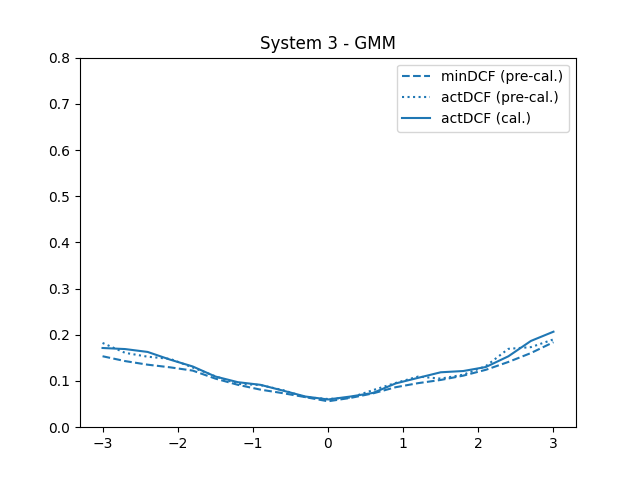
\includegraphics[width=0.4\textwidth]{project11/project11_GMM}}
    \caption{(a) QLR (b) SVM RBF (c) GMM }
    \label{fig:Calibration_all_models}
\end{figure}

We can also plot the Bayes Error and see that the calibration transformation improves our models for every application.

\subsection{Models fusion}
Now, we compute a score-level fusion of these three best-performing models. The values of minDCF and actDCF, for our application, are improved even in respect to our previous best model (GMM).

\begin{table}[ht!]
	\centering
 	\begin{tabular}{| | c c c c | |} 
 		\hline
 		Model & $\pi$ & Min DCF & Act DCF\\
 		\hline\hline
 		Fusion & 0.1 &  0.1277 & 0.1356\\
 		\hline
 	\end{tabular}
	\caption{Model fusion calibration}
\end{table}

Plotting the Bayes error of the three models and their fusion, we see that indeed the fusion is the best one, even if for some application the GMM model could be better in terms of actual DCF.

\begin{figure}[ht]
	\centering
	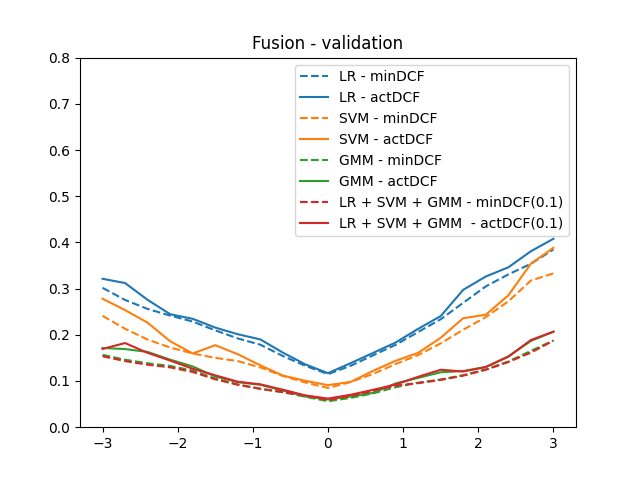
\includegraphics[width=.4\textwidth]{project11/validation}
	\caption{Model Fusion}
	\label{fig:Model_Fusion}
\end{figure}

The scores of the fused model are also well calibrated over the entire range of applications in exam.

For the next part, we'll have to use a model over an evaluation dataset, so we choose the fusion one, because for out application is the best performing one.

\clearpage

\section{Evaluation}
We now evaluate the final delivered system, and perform further analysis to understand whether our design choices were indeed good for our application.

\subsection{Evaluating the fused model}
We consider the fused model and apply it to the evaluation dataset. We observe some performance degradation in respect to the model being applied to the validation dataset used until now, but the relative performance are clearly good: the model is well calibrated for our application and for others too, and the values of minDCF and actDCF are good enough.

\begin{table}[ht!]
	\centering
 	\begin{tabular}{| | c c c c | |} 
 		\hline
 		Model & $\pi$ & Min DCF & Act DCF\\
 		\hline\hline
 		Fusion & 0.1 &  0.1858 & 0.2039\\
 		\hline
 	\end{tabular}
	\caption{Model fusion calibration}
\end{table}

We can visualize its performance across a wide range of applications and appreciate that it is very well calibrated, slightly worse for the upper and lower bounds of the plot.

\begin{figure}[ht]
	\centering
	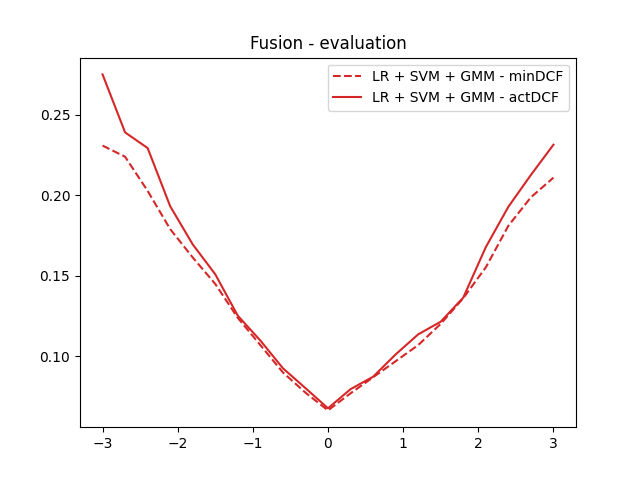
\includegraphics[width=.4\textwidth]{project11/evalFusion}
	\caption{Fusion Model Evaluation}
	\label{fig:Fusion_Model_Evaluation}
\end{figure}

(the scale in this plot is different from the one used on the majority of the others, ndr).

\subsection{Evaluating all the models}

\begin{table}[ht!]
	\centering
 	\begin{tabular}{| | c c c c | |} 
 		\hline
 		Model & Min DCF & Act DCF & \% mis-cal\\
 		\hline\hline
 		QLR & 0.3515 & 0.3684 & 04.81\\
 		\hline
 		SVM & 0.2622 & 0.2879 & 09.80\\
 		\hline
 		GMM & \textbf{0.1838} & 0.2106 & 14.56\\
 		\hline
 		Fusion & 0.1858 & \textbf{0.2039} & 09.77\\
 		\hline
 	\end{tabular}
	\caption{Models evaluation}
\end{table}

We now consider also the other three models and compute their minDCF, actDCF for the target application. We can see that in this case, the GMM model could perform better, since it has a slightly smaller minDCF value, but the fusion model actually performs better.

All the models are also well calibrated, with values of minDCF and actDCF not too different, meaning the models are reaching good performances.

We plot the Bayes errors and we can see that the good performances of the models, like when we did the analysis over the validation dataset, are good over the whole range of applications, not only for our target one.

\begin{figure}[ht]
	\centering
	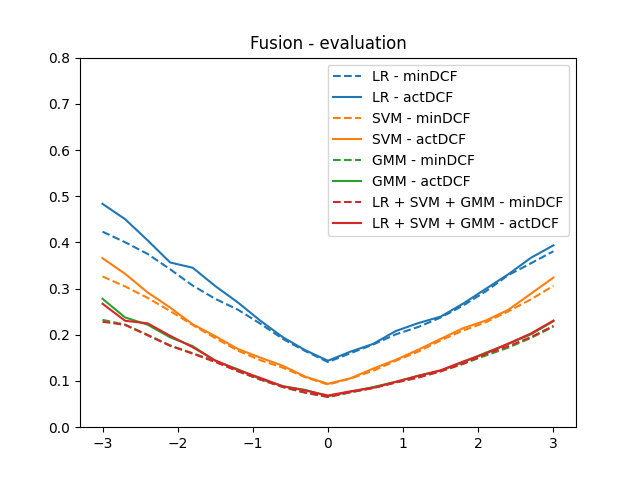
\includegraphics[width=.4\textwidth]{project11/evaluation}
	\caption{All Models Evaluation}
	\label{fig:Model_Evaluation}
\end{figure}

\subsection{Testing different fusion models}
We can try to use different combinations of model to generate our fusion one, and we see that fusing only the SVM and GMM ones could give us better theoretical performances, but the best value of actDCF is obtained using our chosen model, given by the fusion of all threes.

\begin{table}[ht!]
	\centering
 	\begin{tabular}{| | c c c c c | |} 
 		\hline
 		Fusion & $\pi$ & Min DCF & Act DCF & \% mis-cal\\
 		\hline\hline
 		1-2-3 & 0.1 & 0.1858 & \textbf{0.2039} & 09.77\\
 		\hline
 		1-2 & 0.9 & 0.2579 & 0.2844 & 10.26\\
 		\hline
 		2-3 & 0.7 & \textbf{0.1818} & 0.2076 & 14.20\\
 		\hline
 		1-3 & 0.1 &  0.1855 & \textbf{0.2039} & 09.96\\
 		\hline
 	\end{tabular}
	\caption{Model fusion comparison}
\end{table}

\subsection{Trying different hyper-parameter combinations for LR model}
We now choose the Linear Regression model and try to determine if our model selection, applying the model over the evaluation data, was right. 

To do so, we retrain all the principal models (linear, weighted-prior and QLR EF, we choose to not reuse the centered model since we saw on the validation dataset that the results were unchanged).

We then iterate over the same values of lambda we used when we trained those models, and computed minDCF, actDCF and misclassification error. We compare the values of minDCF, since using the actual ones is skewed by the fact that those are not calibrated scores.

In the following page is presented a table holding all the results.
\clearpage

\begin{table}[h]
\centering
\begin{tabular}{|| c  c  c  c  c ||}
\hline
\textbf{$\lambda$} & Model & Min DCF & Act DCF & \% mis-cal \\
\hline\hline
\multirow{3}{*}{0.0001} 
 & Model QLR EF & 0.3545 & 0.3748 & 5.70 \\
 & Model Weight-Prior & 0.5076 & 0.5205 & 2.55 \\
 & Linear & 0.5084 & 0.5125 & 0.80 \\
\hline
\multirow{3}{*}{0.0003}
 & Model QLR EF & 0.3545 & 0.3655 & 3.09 \\
 & Model Weight-Prior & 0.5076 & 0.5139 & 1.25 \\
 & Linear & 0.5088 & 0.5178 & 1.78 \\
\hline
\multirow{3}{*}{0.0010}
 & Model QLR EF & 0.3525 & 0.3663 & 3.92 \\
 & Model Weight-Prior & 0.5076 & 0.5213 & 2.70 \\
 & Linear & 0.5087 & 0.5292 & 4.03 \\
\hline
\multirow{3}{*}{0.0032}
 & Model QLR EF & 0.3527 & 0.3578 & 1.44 \\
 & Model Weight-Prior & 0.5099 & 0.5237 & 2.72 \\
 & Linear & 0.5077 & 0.5198 & 2.37 \\
\hline
\multirow{3}{*}{0.0100}
 & Model QLR EF & \textbf{0.3471} & 0.3756 & 8.22 \\
 & Model Weight-Prior & 0.5101 & 0.5262 & 3.15 \\
 & Linear & 0.5061 & 0.5291 & 4.56 \\
\hline
\multirow{3}{*}{0.0316}
 & Model QLR EF & 0.3515 & 0.4922 & 40.04 \\
 & Model Weight-Prior & 0.5095 & 0.6305 & 23.77 \\
 & Linear & 0.5054 & 0.6158 & 21.85 \\
\hline
\multirow{3}{*}{0.1000}
 & Model QLR EF & 0.3596 & 0.7284 & 102.57 \\
 & Model Weight-Prior & 0.5071 & 0.9167 & 80.79 \\
 & Linear & 0.5074 & 0.8391 & 65.37 \\
\hline
\multirow{3}{*}{0.3162}
 & Model QLR EF & 0.3719 & 0.9632 & 159.02 \\
 & Model Weight-Prior & 0.5061 & 1.0000 & 97.60 \\
 & Linear & 0.5058 & 0.9953 & 96.80 \\
\hline
\multirow{3}{*}{1.0000}
 & Model QLR EF & 0.4011 & 0.9987 & 149.00 \\
 & Model Weight-Prior & 0.5081 & 1.0000 & 96.82 \\
 & Linear & 0.5061 & 1.0000 & 97.60 \\
\hline
\multirow{3}{*}{3.1623}
 & Model QLR EF & 0.4291 & 1.0000 & 133.05 \\
 & Model Weight-Prior & 0.5091 & 1.0000 & 96.44 \\
 & Linear & 0.5084 & 1.0000 & 96.69 \\
\hline
\multirow{3}{*}{10.0000}
 & Model QLR EF & 0.4416 & 1.0000 & 126.45 \\
 & Model Weight-Prior & 0.5091 & 1.0000 & 96.44 \\
 & Linear & 0.5091 & 1.0000 & 96.44 \\
\hline
\multirow{3}{*}{31.6228}
 & Model QLR EF & 0.4436 & 1.0000 & 125.43 \\
 & Model Weight-Prior & 0.5091 & 1.0000 & 96.44 \\
 & Linear & 0.5091 & 1.0000 & 96.44 \\
\hline
\multirow{3}{*}{100.0000}
 & Model QLR EF & 0.4476 & 1.0000 & 123.40 \\
 & Model Weight-Prior & 0.5091 & 1.0000 & 96.44 \\
 & Linear & 0.5091 & 1.0000 & 96.44 \\
\hline
\end{tabular}
\caption{Comparison of Model Performance for Different $\lambda$ Values}
\label{tab:model-comparison}
\end{table}
\clearpage

The best model is still the quadratic one, but we find a different best value for $\lambda$ = 0.01 (we used 0.03126).

From this table, we can very well see that incrementing the value of $\lambda$ over 0.1 make all three models perform very poorly, likely due to excessive regularization and poor generalization on the evaluation set.

In conclusion, we chose the right model - for the LR one, at least - with a not so optimal value of the regularization parameter - though it still gave us the third best minDCF - at least considering our application. We could try to calibrate the scores since smaller values of minDCF does not mean that also the actDCF will be the lowest.

\end{document}